\documentclass[english,floatsintext,man]{apa6}

\usepackage{amssymb,amsmath}
\usepackage{ifxetex,ifluatex}
\usepackage{fixltx2e} % provides \textsubscript
\ifnum 0\ifxetex 1\fi\ifluatex 1\fi=0 % if pdftex
  \usepackage[T1]{fontenc}
  \usepackage[utf8]{inputenc}
\else % if luatex or xelatex
  \ifxetex
    \usepackage{mathspec}
    \usepackage{xltxtra,xunicode}
  \else
    \usepackage{fontspec}
  \fi
  \defaultfontfeatures{Mapping=tex-text,Scale=MatchLowercase}
  \newcommand{\euro}{€}
\fi
% use upquote if available, for straight quotes in verbatim environments
\IfFileExists{upquote.sty}{\usepackage{upquote}}{}
% use microtype if available
\IfFileExists{microtype.sty}{\usepackage{microtype}}{}

% Table formatting
\usepackage{longtable, booktabs}
\usepackage{lscape}
% \usepackage[counterclockwise]{rotating}   % Landscape page setup for large tables
\usepackage{multirow}		% Table styling
\usepackage{tabularx}		% Control Column width
\usepackage[flushleft]{threeparttable}	% Allows for three part tables with a specified notes section
\usepackage{threeparttablex}            % Lets threeparttable work with longtable

% Create new environments so endfloat can handle them
% \newenvironment{ltable}
%   {\begin{landscape}\begin{center}\begin{threeparttable}}
%   {\end{threeparttable}\end{center}\end{landscape}}

\newenvironment{lltable}
  {\begin{landscape}\begin{center}\begin{ThreePartTable}}
  {\end{ThreePartTable}\end{center}\end{landscape}}




% The following enables adjusting longtable caption width to table width
% Solution found at http://golatex.de/longtable-mit-caption-so-breit-wie-die-tabelle-t15767.html
\makeatletter
\newcommand\LastLTentrywidth{1em}
\newlength\longtablewidth
\setlength{\longtablewidth}{1in}
\newcommand\getlongtablewidth{%
 \begingroup
  \ifcsname LT@\roman{LT@tables}\endcsname
  \global\longtablewidth=0pt
  \renewcommand\LT@entry[2]{\global\advance\longtablewidth by ##2\relax\gdef\LastLTentrywidth{##2}}%
  \@nameuse{LT@\roman{LT@tables}}%
  \fi
\endgroup}


  \usepackage{graphicx}
  \makeatletter
  \def\maxwidth{\ifdim\Gin@nat@width>\linewidth\linewidth\else\Gin@nat@width\fi}
  \def\maxheight{\ifdim\Gin@nat@height>\textheight\textheight\else\Gin@nat@height\fi}
  \makeatother
  % Scale images if necessary, so that they will not overflow the page
  % margins by default, and it is still possible to overwrite the defaults
  % using explicit options in \includegraphics[width, height, ...]{}
  \setkeys{Gin}{width=\maxwidth,height=\maxheight,keepaspectratio}
\ifxetex
  \usepackage[setpagesize=false, % page size defined by xetex
              unicode=false, % unicode breaks when used with xetex
              xetex]{hyperref}
\else
  \usepackage[unicode=true]{hyperref}
\fi
\hypersetup{breaklinks=true,
            pdfauthor={},
            pdftitle={Project 3: Sea Port Program},
            colorlinks=true,
            citecolor=blue,
            urlcolor=blue,
            linkcolor=black,
            pdfborder={0 0 0}}
\urlstyle{same}  % don't use monospace font for urls

\setlength{\parindent}{0pt}
%\setlength{\parskip}{0pt plus 0pt minus 0pt}

\setlength{\emergencystretch}{3em}  % prevent overfull lines

\ifxetex
  \usepackage{polyglossia}
  \setmainlanguage{}
\else
  \usepackage[english]{babel}
\fi

% Manuscript styling
\captionsetup{font=singlespacing,justification=justified}
\usepackage{csquotes}
\usepackage{upgreek}



\usepackage{tikz} % Variable definition to generate author note

% fix for \tightlist problem in pandoc 1.14
\providecommand{\tightlist}{%
  \setlength{\itemsep}{0pt}\setlength{\parskip}{0pt}}

% Essential manuscript parts
  \title{Project 3: Sea Port Program}

  \shorttitle{Project 3}


  \author{Justin VanWinkle}

  \def\affdep{{""}}%
  \def\affcity{{""}}%

  \affiliation{
    \vspace{0.5cm}
          \textsuperscript{} 23 April 2017  }

 % If no author_note is defined give only author information if available
    \authornote{
    \newcounter{author}
                        }
  

  




\begin{document}

\maketitle

\setcounter{secnumdepth}{0}



\section{Design}\label{design}

From a high level, this program has been built with a class that
contains the UI separate from any workflow logic. This paves the way for
several simplistic approaches when concurrency is included into the
program in a future iteration. One such example would be creating the
world using a thread that is separate from that of the Event Dispatch
Thread that would be used by default when calling a function from an
event listener that is attached to a swing component. Such a separation
becomes easily manageable when business logic and view logic remain
isolated.

\subsection{Decisions}\label{decisions}

\begin{itemize}
\tightlist
\item
  I chose not to use the comparable interface on the Thing class,
  because I don't believe it is needed and I don't want dead code.
\item
  TDD was used for some areas of the program to ensure that changes in
  future iterations do not alter the functionality of those methods.
\item
  A map was used in the World class to track all objects for two main
  reasons. First, the complexity of creating the model is greatly
  reduced since parent objects can be found without having to search for
  them. Second, this allows for O(n) lookup time for any object that
  exists in the World. So for the purposes of this class, the time
  needed to create the World is drastically reduced -- especially for
  very large input files.
\item
  Each class that uses a thread is left as responsible for its own
  thread. This wasn't as much of a decision as it was a convention.
\end{itemize}

\subsection{Meanings}\label{meanings}

The various classes, packages, variables, and methods in this program
are organized in a logical manner that show good practices in
object-oriented design. Each of the items has been placed in such a way
that it has some sort of direct relationship with its containing parent
or its contained child.

\subsubsection{Classes}\label{classes}

All classes assume no knowledge of their calling class whether by
passing context or interface. This is likely to change in a future
iteration, however.

\paragraph{\texorpdfstring{The \emph{Thing}
Package}{The Thing Package}}\label{the-thing-package}

Each class in the \emph{thing} package as well as classes in the sub
packages of \emph{thing} represent real world objects that reflect their
name.

\paragraph{Other Classes}\label{other-classes}

The PortTime class, in a similar manner represents the time of a port.
Due to ambiguous requirements, however, the developer was unable to
determine the intended use of this class. Therefore, it is assumed that
this class will be better integrated in a future iteration.

\subsubsection{Variables}\label{variables}

In each class, there are sets of instance variables that represent a
\emph{has-a} relationship between the class and the item that variable
holds. For instance, a SeaPort has a (or many) Dock(s).

\subsection{Methods}\label{methods}

The SeaPortProgram class contains the heart of creating the world
including all of the logic for parsing out the input file, creating the
objects, and modeling a world that represents what is defined in the
input file. While the requirement documentation \emph{suggests} that a
scanner should be used, a string tokenizer was used instead. While this
adds some additional coding overhead,

\section{User's Guide}\label{users-guide}

This serves as a guide for all you need to know to get up and running
with this program

\subsection{How to start the program}\label{how-to-start-the-program}

To compile, cd into the src directory and run the command
\texttt{javac\ *.java\ */*.java\ */*/*.java}. Once that command has
completed, run
\texttt{java\ -classpath\ \textless{}path-to-src-folder\textgreater{}\ main.SeaPortProgram}.

\subsection{How to create a world}\label{how-to-create-a-world}

\begin{enumerate}
\def\labelenumi{\arabic{enumi}.}
\tightlist
\item
  Click \enquote{Select File}.
\item
  Navigate to and select a valid input file.
\item
  Select \enquote{Open}.
\item
  World is automatically modeled. Notice the output that matches the
  data in the chosen input file.
\end{enumerate}

\subsection{Search}\label{search}

Searches using regex provide the user with more control over the
matching pattern. Matches look at three criteria: name, index, and
skill.

\subsubsection{How to search}\label{how-to-search}

\begin{enumerate}
\def\labelenumi{\arabic{enumi}.}
\tightlist
\item
  Input a valid java regex engine pattern in the search box. (Valid
  regex patterns for the java regex engine can be obtained
  \href{http://docs.oracle.com/javase/8/docs/api/java/util/regex/Pattern.html}{here}.
\item
  Click \enquote{Search}. Searching returns a list of all \emph{Things}
  that have a Name or Index that match the criteria. Some additional
  cases exist such as searching the skills of a Person or the duration
  of a Job.
\end{enumerate}

\subsubsection{Examples}\label{examples}

\begin{itemize}
\tightlist
\item
  Search Pattern: \enquote{ar}

  \begin{itemize}
  \tightlist
  \item
    Matches \enquote{Sara}
  \item
    Does not Match \enquote{Archie}
  \end{itemize}
\item
  Search Pattern: \enquote{{[}A\textbar{}a{]}r}

  \begin{itemize}
  \tightlist
  \item
    Matches \enquote{Sara} and \enquote{Archie} For more extended
    documentation on regex patterns,
    \href{http://docs.oracle.com/javase/8/docs/api/java/util/regex/Pattern.html}{go
    here}.
  \end{itemize}
\end{itemize}

\subsection{Sorting}\label{sorting}

Sorting can be done on all lists and sub lists in the program. For
convenience, the sort dialog will remain open until the user closes it.

\subsubsection{How to sort}\label{how-to-sort}

\begin{enumerate}
\def\labelenumi{\arabic{enumi}.}
\tightlist
\item
  Once a file has loaded, the \texttt{sort} button can be clicked which
  will open a sort picking dialog.
\item
  On the sort picking dialog, select the desired sort options and click
  \texttt{sort}.
\item
  Repeat until the desired sorts are achieved.
\end{enumerate}

\subsubsection{How to cancel or suspend a
job}\label{how-to-cancel-or-suspend-a-job}

\emph{Note}: Cancelled jobs are handled similar to a completed job, but
have no additional effort applied. This allows the ship to undock. 1.
While jobs are running, click \enquote{Suspend} or \enquote{Cancel}. 2.
Enter the index of the job you wish to interact with. 3. Click
\enquote{Ok} and note that the job has stopped progressing.

\subsection{Special Features}\label{special-features}

The JTree automatically refreshes its Ship and Job nodes to show
progress in a near-realtime manner. If a new file is loaded, the JTree
abandoned and reloaded with the new incoming data model.

\section{Test Plan}\label{test-plan}

\begin{enumerate}
\def\labelenumi{\arabic{enumi}.}
\tightlist
\item
  Base Case

  \begin{itemize}
  \tightlist
  \item
    \textbf{Input:} (1.txt) Using the input file outlined in the
    requirements documentation
  \item
    \textbf{Expected:} Ouput that matches the output outlined in the
    documentation. And All ships will be immediately undocked.
  \item
    \textbf{Result:} An exact match between the expected output and the
    actual output. And all ships are immediately undocked.
  \end{itemize}
\item
  Very large input file

  \begin{itemize}
  \tightlist
  \item
    \textbf{Input:} (2.txt) Using an input file that is extremely large
    to ensure no allocation issues
  \item
    \textbf{Expected:} No errors and output that displays an appropriate
    data structure to match the input.
  \item
    \textbf{Result:} An out of memory error is thrown and no further
    actions are completed by the program. This is caused by the OS
    limitation on the number of threads it will allow to be thrown on
    the allocated heap.
  \end{itemize}
\item
  Searching \enquote{ar}

  \begin{itemize}
  \tightlist
  \item
    \textbf{Input:} (1.txt) Containing names with
    \texttt{\textbackslash{}*ar\textbackslash{}*} and
    \texttt{Ar\textbackslash{}*}.
  \item
    \textbf{Expected:} Matches with names only containing
    \texttt{\textbackslash{}*ar\textbackslash{}*}.
  \item
    \textbf{Result:} Search returns only names that contain
    \texttt{\textbackslash{}*ar\textbackslash{}*}. (See figure 1)
  \end{itemize}
\item
  Sorting All Ascending by name

  \begin{itemize}
  \tightlist
  \item
    \textbf{Input:} (4.txt) An input file containing multiple ports.
  \item
    \textbf{Expected:} All items in the tree will be sorted in ascending
    order by name.
  \item
    \textbf{Result:} All items are sorted in ascending order in the
    tree. (See figure 2)
  \end{itemize}
\item
  Unit tests

  \begin{itemize}
  \tightlist
  \item
    Unit tests were written to ensure that units of code perform the
    same basic function even after changes are made.
  \item
    \textbf{Expected:} All unit tests should pass.
  \item
    \textbf{Result:} All unit tests pass.
  \end{itemize}
\item
  Small Data Set

  \begin{itemize}
  \tightlist
  \item
    \textbf{Input} (4.txt) An input file containing a small set of data
  \item
    \textbf{Expected:} All jobs will progress to completion and docked
    ships will be replaced with ships in que.
  \item
    \textbf{Result:} All ships have all jobs completed while docked.
  \end{itemize}
\item
  Large Data Set

  \begin{itemize}
  \tightlist
  \item
    \textbf{Input} (3.txt) An input file containing a relatively large
    set of data
  \item
    \textbf{Expected:} All jobs will progress to completion and docked
    ships will be replaced with ships in que.
  \item
    \textbf{Result:} All ships have all jobs completed while docked.
  \end{itemize}
\end{enumerate}

\section{Lessons Learned}\label{lessons-learned}

In the coming sections, consideration will be given to particular pain
points, gleanings, and takeaways.

\subsection{Concurrency}\label{concurrency}

I haven't worked with concurrency in Java for several years. Having said
that, I have been using GoLang at work for the past year and have come
to love the implementations of the libs surrounding concurrency -- so
much so that it was painful to not have go routines and channels. Java
has, however, become slightly nicer in this area with the introduction
of lambda functions. I haven't looked into it, but it almost makes me
think that functions can be handled as first-class citizens in Java now.
I'd be interested to know!

\subsection{About This Documentation}\label{about-this-documentation}

Since discovering Pandoc, I have written all of my professional
documentation and papers in markdown and used Pandoc to convert them to
whatever end format I require. Markdown allows me to focus on content
rather than formatting and thus saves great amounts of time. One
particular hurdle in writing this documentation was finding a way to use
\LaTeX~to handle the formatting in a way that was consistent with the
APA style guide. As a result, I came across a set of tools that allows
me to continue using Pandoc to pipe everything through a template that
\LaTeX~uses to ultimately format my paper perfectly according to the APA
style -- and all I ever did was write this in markdown with some yaml
front matter. A glorious combination when paired with Vim.

\subsection{New Classes Used}\label{new-classes-used}

\subsubsection{JScrollPane}\label{jscrollpane}

While I purposefully avoid Java's built in UI libraries, it came as no
surprise when I found myself using the JScrollPane class for the first
time in this program. I did find JScrollPane to be comparatively easy to
work with for the sake of just getting a scroll view set up.

\subsubsection{JTree}\label{jtree}

I found JTree to be easy to work with and rather intuitive. It did force
me to refactor all of my \texttt{toString()} methods -- but for the
better. JTree has proven to be quite painful when working with
concurrency. Since it is modeling a wide array of data, it is easy to
miss a section that should be synchronized.

\subsubsection{JSplitPane}\label{jsplitpane}

Once again, easy and intuitive. I don't quite like JSplitPane, however,
because I feel that it paves the way for a bad UX. That's purely opinion
at this point, though.

\subsection{Future Iterations}\label{future-iterations}

Project 1: In a future iteration, I would like to focus on pushing all
UI driven events to the EDT and all other tasks onto other threads. In
the words of Vern Gosdin, \enquote{This ain't my first rodeo.}
Additionally, I would likely opt for some sort of utility class if too
much begins to be repeated among the various classes. I already see
where this might be possible as the search expands and I could offload
the matching to a static utility method that just grabs the specified
fields from each of the classes for comparison. Thing implements the
comparable interface, but makes no actual use of the interface.
Currently, the compareTo() method is overridden in Thing, but in the
future, Thing need to be an abstract class and all subclasses will need
to override this comparable method. Lastly, there is plenty of room for
additional unit tests. New unit tests should be written on any logic
code before any alterations are made for concurrency to ensure proper
results.

Project 2: The main UI class is getting cumbersome. I would like to see
it be split out into a second class as appropriate. The two UI classes
have some repetitive code that could go into a static method of a
utility class. The search could allow for more robust options such as
searching only on Persons.

Project 3: Similar to the previous project, I feel that the primary UI
file is getting very cumbersome. While it is fairly well split into
functional areas, it is calling desperately for a refactor to place
actions and utils into a util class. Some additional work should also be
done to clean up some small bugs with the JTree not rendering the nodes
properly. I think this could be fixed by using an invokeLater() or using
a graphics buffer.

\section{Figures}\label{figures}

\begin{figure}[htbp]
\centering
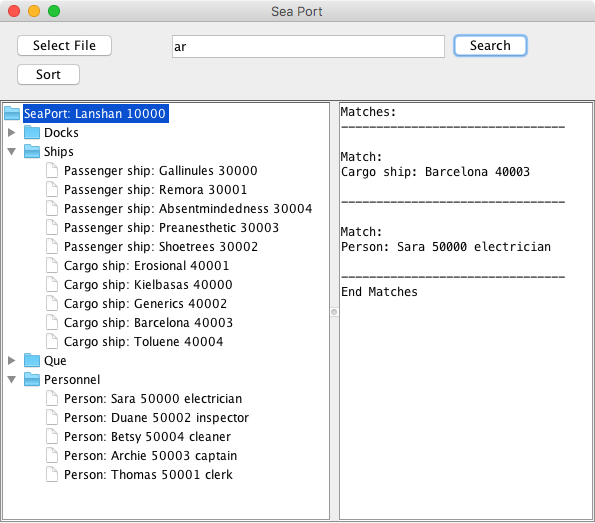
\includegraphics{/Users/vanwinklej/workspace/UMUC/oop-concurrency/project/doc/p2search.png}
\caption{Search Test}
\end{figure}

\begin{figure}[htbp]
\centering
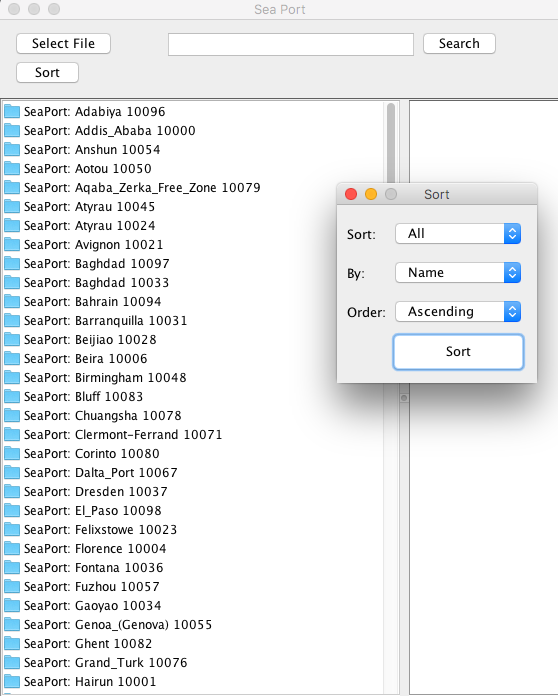
\includegraphics{/Users/vanwinklej/workspace/UMUC/oop-concurrency/project/doc/p2sort.png}
\caption{Sort Test}
\end{figure}

\begin{figure}[htbp]
\centering
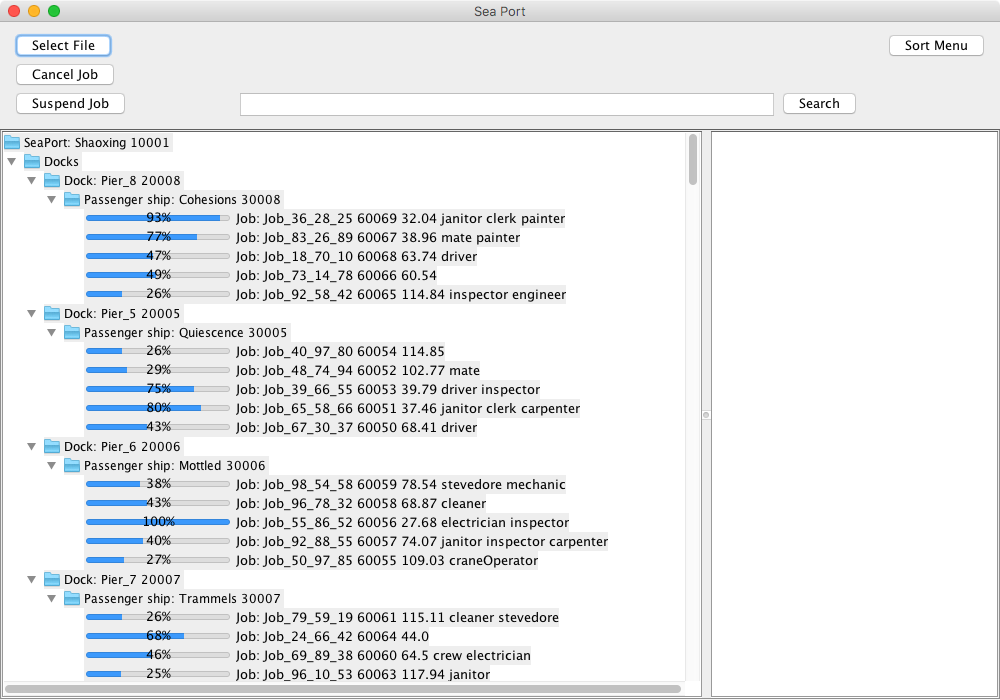
\includegraphics{/Users/vanwinklej/workspace/UMUC/oop-concurrency/project/doc/3running.png}
\caption{Running Jobs}
\end{figure}

\begin{figure}[htbp]
\centering
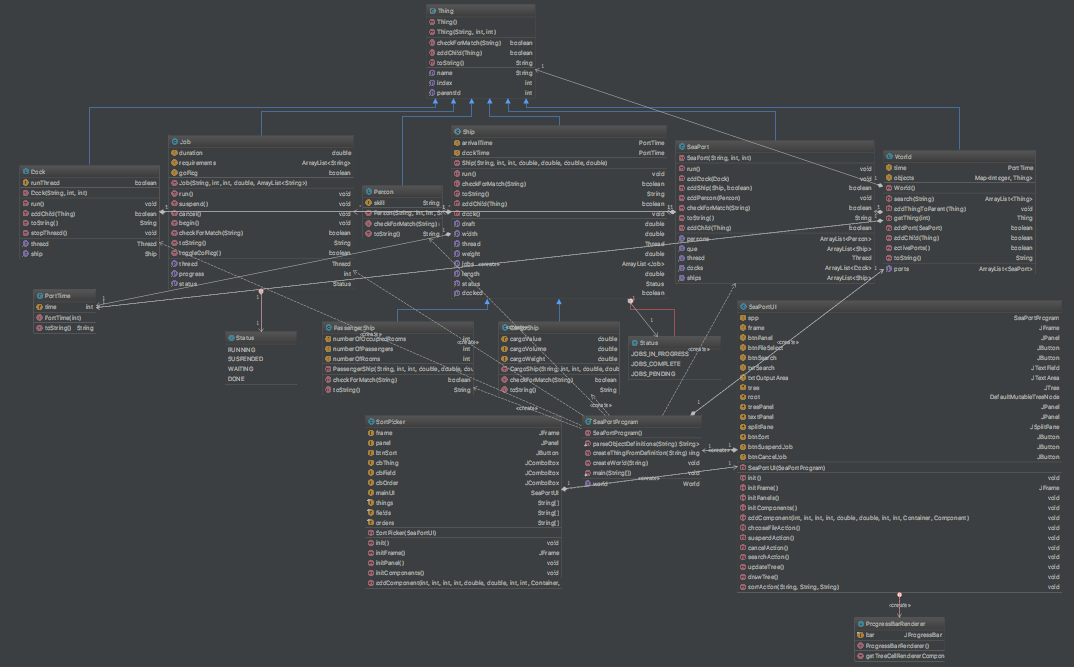
\includegraphics{/Users/vanwinklej/workspace/UMUC/oop-concurrency/project/doc/diagram.png}
\caption{UML Diagram}
\end{figure}

\setlength{\parindent}{-0.5in} \setlength{\leftskip}{0.5in}






\end{document}
